\documentclass[twoside]{book}

% Packages required by doxygen
\usepackage{fixltx2e}
\usepackage{calc}
\usepackage{doxygen}
\usepackage[export]{adjustbox} % also loads graphicx
\usepackage{graphicx}
\usepackage[utf8]{inputenc}
\usepackage{makeidx}
\usepackage{multicol}
\usepackage{multirow}
\PassOptionsToPackage{warn}{textcomp}
\usepackage{textcomp}
\usepackage[nointegrals]{wasysym}
\usepackage[table]{xcolor}

% Font selection
\usepackage[T1]{fontenc}
\usepackage[scaled=.90]{helvet}
\usepackage{courier}
\usepackage{amssymb}
\usepackage{sectsty}
\renewcommand{\familydefault}{\sfdefault}
\allsectionsfont{%
  \fontseries{bc}\selectfont%
  \color{darkgray}%
}
\renewcommand{\DoxyLabelFont}{%
  \fontseries{bc}\selectfont%
  \color{darkgray}%
}
\newcommand{\+}{\discretionary{\mbox{\scriptsize$\hookleftarrow$}}{}{}}

% Page & text layout
\usepackage{geometry}
\geometry{%
  a4paper,%
  top=2.5cm,%
  bottom=2.5cm,%
  left=2.5cm,%
  right=2.5cm%
}
\tolerance=750
\hfuzz=15pt
\hbadness=750
\setlength{\emergencystretch}{15pt}
\setlength{\parindent}{0cm}
\setlength{\parskip}{3ex plus 2ex minus 2ex}
\makeatletter
\renewcommand{\paragraph}{%
  \@startsection{paragraph}{4}{0ex}{-1.0ex}{1.0ex}{%
    \normalfont\normalsize\bfseries\SS@parafont%
  }%
}
\renewcommand{\subparagraph}{%
  \@startsection{subparagraph}{5}{0ex}{-1.0ex}{1.0ex}{%
    \normalfont\normalsize\bfseries\SS@subparafont%
  }%
}
\makeatother

% Headers & footers
\usepackage{fancyhdr}
\pagestyle{fancyplain}
\fancyhead[LE]{\fancyplain{}{\bfseries\thepage}}
\fancyhead[CE]{\fancyplain{}{}}
\fancyhead[RE]{\fancyplain{}{\bfseries\leftmark}}
\fancyhead[LO]{\fancyplain{}{\bfseries\rightmark}}
\fancyhead[CO]{\fancyplain{}{}}
\fancyhead[RO]{\fancyplain{}{\bfseries\thepage}}
\fancyfoot[LE]{\fancyplain{}{}}
\fancyfoot[CE]{\fancyplain{}{}}
\fancyfoot[RE]{\fancyplain{}{\bfseries\scriptsize Generated by Doxygen }}
\fancyfoot[LO]{\fancyplain{}{\bfseries\scriptsize Generated by Doxygen }}
\fancyfoot[CO]{\fancyplain{}{}}
\fancyfoot[RO]{\fancyplain{}{}}
\renewcommand{\footrulewidth}{0.4pt}
\renewcommand{\chaptermark}[1]{%
  \markboth{#1}{}%
}
\renewcommand{\sectionmark}[1]{%
  \markright{\thesection\ #1}%
}

% Indices & bibliography
\usepackage{natbib}
\usepackage[titles]{tocloft}
\setcounter{tocdepth}{3}
\setcounter{secnumdepth}{5}
\makeindex

% Hyperlinks (required, but should be loaded last)
\usepackage{ifpdf}
\ifpdf
  \usepackage[pdftex,pagebackref=true]{hyperref}
\else
  \usepackage[ps2pdf,pagebackref=true]{hyperref}
\fi
\hypersetup{%
  colorlinks=true,%
  linkcolor=blue,%
  citecolor=blue,%
  unicode%
}

% Custom commands
\newcommand{\clearemptydoublepage}{%
  \newpage{\pagestyle{empty}\cleardoublepage}%
}

\usepackage{caption}
\captionsetup{labelsep=space,justification=centering,font={bf},singlelinecheck=off,skip=4pt,position=top}

%===== C O N T E N T S =====

\begin{document}

% Titlepage & ToC
\hypersetup{pageanchor=false,
             bookmarksnumbered=true,
             pdfencoding=unicode
            }
\pagenumbering{alph}
\begin{titlepage}
\vspace*{7cm}
\begin{center}%
{\Large libc-\/template }\\
\vspace*{1cm}
{\large Generated by Doxygen 1.8.13}\\
\end{center}
\end{titlepage}
\clearemptydoublepage
\pagenumbering{roman}
\tableofcontents
\clearemptydoublepage
\pagenumbering{arabic}
\hypersetup{pageanchor=true}

%--- Begin generated contents ---
\chapter{File Index}
\section{File List}
Here is a list of all documented files with brief descriptions\+:\begin{DoxyCompactList}
\item\contentsline{section}{include/\hyperlink{example_8h}{example.\+h} \\*File containing example of doxygen usage for quick reference }{\pageref{example_8h}}{}
\end{DoxyCompactList}

\chapter{File Documentation}
\hypertarget{example_8h}{}\section{include/example.h File Reference}
\label{example_8h}\index{include/example.\+h@{include/example.\+h}}


File containing example of doxygen usage for quick reference.  


{\ttfamily \#include $<$stdlib.\+h$>$}\newline
{\ttfamily \#include $<$stdio.\+h$>$}\newline
{\ttfamily \#include $<$assert.\+h$>$}\newline
Include dependency graph for example.\+h\+:
\nopagebreak
\begin{figure}[H]
\begin{center}
\leavevmode
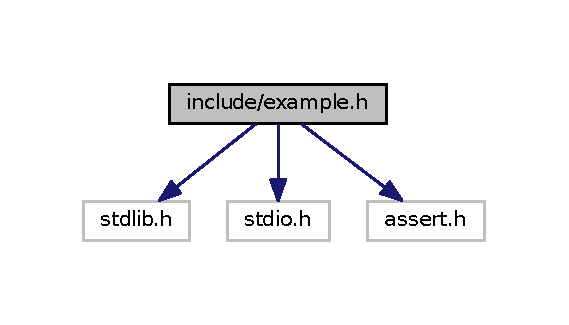
\includegraphics[width=273pt]{example_8h__incl}
\end{center}
\end{figure}
\subsection*{Macros}
\begin{DoxyCompactItemize}
\item 
\#define \hyperlink{example_8h_a0acb682b8260ab1c60b918599864e2e5}{T}~Example\+\_\+T
\begin{DoxyCompactList}\small\item\em An example of an opaque structure. \end{DoxyCompactList}\end{DoxyCompactItemize}
\subsection*{Typedefs}
\begin{DoxyCompactItemize}
\item 
\mbox{\Hypertarget{example_8h_a24514489b0962fafe8414bfae95aa268}\label{example_8h_a24514489b0962fafe8414bfae95aa268}} 
typedef struct T $\ast$ {\bfseries T}
\end{DoxyCompactItemize}
\subsection*{Functions}
\begin{DoxyCompactItemize}
\item 
\hyperlink{example_8h_a0acb682b8260ab1c60b918599864e2e5}{T} \hyperlink{example_8h_a29e75ca11a9801d424f5daebd3f727b6}{Example\+\_\+new} (void)
\begin{DoxyCompactList}\small\item\em Instantiates the object. \end{DoxyCompactList}\item 
void \hyperlink{example_8h_a7e0cb3c855a7b47018983f51ec8fb866}{Example\+\_\+free} (\hyperlink{example_8h_a0acb682b8260ab1c60b918599864e2e5}{T} $\ast$ex)
\begin{DoxyCompactList}\small\item\em Frees the object. \end{DoxyCompactList}\end{DoxyCompactItemize}


\subsection{Detailed Description}
File containing example of doxygen usage for quick reference. 

\begin{DoxyAuthor}{Author}
Cody Luu Here typically goes a more extensive explanation of what the header defines. Doxygens tags are words preceeded by either a backslash \textbackslash{} or by an at symbol @. 
\end{DoxyAuthor}
\begin{DoxySeeAlso}{See also}
\href{http://fnch.users.sourceforge.net/doxygen_c.html}{\tt http\+://fnch.\+users.\+sourceforge.\+net/doxygen\+\_\+c.\+html} 
\end{DoxySeeAlso}


\subsection{Macro Definition Documentation}
\mbox{\Hypertarget{example_8h_a0acb682b8260ab1c60b918599864e2e5}\label{example_8h_a0acb682b8260ab1c60b918599864e2e5}} 
\index{example.\+h@{example.\+h}!T@{T}}
\index{T@{T}!example.\+h@{example.\+h}}
\subsubsection{\texorpdfstring{T}{T}}
{\footnotesize\ttfamily \#define T~Example\+\_\+T}



An example of an opaque structure. 

It uses two levels of indirection, I think. 

\subsection{Function Documentation}
\mbox{\Hypertarget{example_8h_a7e0cb3c855a7b47018983f51ec8fb866}\label{example_8h_a7e0cb3c855a7b47018983f51ec8fb866}} 
\index{example.\+h@{example.\+h}!Example\+\_\+free@{Example\+\_\+free}}
\index{Example\+\_\+free@{Example\+\_\+free}!example.\+h@{example.\+h}}
\subsubsection{\texorpdfstring{Example\+\_\+free()}{Example\_free()}}
{\footnotesize\ttfamily void Example\+\_\+free (\begin{DoxyParamCaption}\item[{\hyperlink{example_8h_a0acb682b8260ab1c60b918599864e2e5}{T} $\ast$}]{ex }\end{DoxyParamCaption})}



Frees the object. 


\begin{DoxyParams}{Parameters}
{\em ex} & The opaque handle we want to free. 
\begin{DoxyCode}
\hyperlink{example_8h_a7e0cb3c855a7b47018983f51ec8fb866}{Example\_free}(ex);
\end{DoxyCode}
 \\
\hline
\end{DoxyParams}
\mbox{\Hypertarget{example_8h_a29e75ca11a9801d424f5daebd3f727b6}\label{example_8h_a29e75ca11a9801d424f5daebd3f727b6}} 
\index{example.\+h@{example.\+h}!Example\+\_\+new@{Example\+\_\+new}}
\index{Example\+\_\+new@{Example\+\_\+new}!example.\+h@{example.\+h}}
\subsubsection{\texorpdfstring{Example\+\_\+new()}{Example\_new()}}
{\footnotesize\ttfamily \hyperlink{example_8h_a0acb682b8260ab1c60b918599864e2e5}{T} Example\+\_\+new (\begin{DoxyParamCaption}\item[{void}]{ }\end{DoxyParamCaption})}



Instantiates the object. 


\begin{DoxyCode}
Example\_t ex = \hyperlink{example_8h_a29e75ca11a9801d424f5daebd3f727b6}{Example\_new}();
\end{DoxyCode}
 
%--- End generated contents ---

% Index
\backmatter
\newpage
\phantomsection
\clearemptydoublepage
\addcontentsline{toc}{chapter}{Index}
\printindex

\end{document}
